\documentclass{article}
\usepackage{float}

\usepackage{lmodern}  % 或者 cm-super
\usepackage[T1]{fontenc}  % 让 LaTeX 使用 T1 字体编码
\usepackage[utf8]{inputenc}  % 确保使用 UTF-8 编码
\usepackage{amsmath} % 数学包
\usepackage{graphicx} % 图形包
\usepackage[colorlinks=true, linkcolor=blue, urlcolor=blue, citecolor=blue]{hyperref}
% 超链接包
\usepackage[a4paper, margin=1in]{geometry}
\usepackage{listings} %可以插入代码
\usepackage{xcolor} %可以定义颜色

\title{Homework1}
\author{Ruilong Chen}
\date{\today}
\setlength{\parindent}{0pt}  % 取消缩进
\setlength{\parskip}{1em}    % 增加段落之间的空行
% 定义颜色
\definecolor{lightgray}{rgb}{0.95, 0.95, 0.95}  % 背景色
\definecolor{keywordcolor}{rgb}{0.2, 0.5, 0.8}   % 关键字颜色
\definecolor{commentcolor}{rgb}{0.5, 0.5, 0.5}   % 注释颜色
\definecolor{stringcolor}{rgb}{0.9, 0.4, 0.4}    % 字符串颜色
\definecolor{numbercolor}{rgb}{0.8, 0.5, 0.2}    % 数字颜色

\lstset{
  language=Python,                            % 设置语言为 Python
  basicstyle=\ttfamily\small,                 % 使用等宽字体,并设置为小号
  numbers=left,                               % 行号显示在左侧
  numberstyle=\tiny\color{gray},              % 行号的字体和颜色
  frame=single,                               % 在代码块周围添加边框
  backgroundcolor=\color{lightgray},          % 背景颜色
  keywordstyle=\color{keywordcolor}\bfseries, % 关键字颜色
  commentstyle=\color{commentcolor}\itshape,  % 注释颜色
  stringstyle=\color{stringcolor},            % 字符串颜色
  numbersep=5pt,                              % 行号与代码之间的间距
  tabsize=4,                                  % 制表符大小
  breaklines=true,                            % 启用自动换行
  breakindent=0pt,                            % 换行后无缩进
  postbreak=\mbox{\textcolor{red}{$\hookrightarrow$}\space}, % 换行时的符号
  escapeinside={(*@}{@*},                      % 允许在代码中使用 LaTeX
  showspaces=false,                           % 不显示空格
  showstringspaces=false                       % 不显示字符串中的空格
}

\begin{document}
\maketitle %之前定义的title展示出来

\section{Question1}

In 1990, Michael Crichton published the book ``Jurassic Park'' about the resurrection of dinosaurs using the blood from the stomachs of insects which had been encased in tree sap, later turned into the mineral, amber. 

At one point in the book, Dr. Henry Wu is asked to explain some of DNA techniques used in reconstructing the extinct dinosaur genomes. Dr. Wu describes the use of restriction enzymes and how the fragmented pieces of dino DNA can be spliced together with these enzymes. He also alludes to the fact that they don't have the entire genome but that they ``fill in the gap'' with modern day frog DNA. 

At one point during his discussion he points to a computer screen and remarks ``Here you see the actual structure of a small fragment of dinosaur DNA.''

>JurassicPark DinoDNA from the book Jurassic Park


gcgttgctgg cgtttttcca taggctccgc ccccctgacg agcatcacaa aaatcgacgc\\
ggtggcgaaa cccgacagga ctataaagat accaggcgtt tccccctgga agctccctcg\\
tgttccgacc ctgccgctta ccggatacct gtccgccttt ctcccttcgg gaagcgtggc\\
tgctcacgct gtaggtatct cagttcggtg taggtcgttc gctccaagct gggctgtgtg\\
ccgttcagcc cgaccgctgc gccttatccg gtaactatcg tcttgagtcc aacccggtaa\\
agtaggacag gtgccggcag cgctctgggt cattttcggc gaggaccgct ttcgctggag\\
atcggcctgt cgcttgcggt attcggaatc ttgcacgccc tcgctcaagc cttcgtcact\\
ccaaacgttt cggcgagaag caggccatta tcgccggcat ggcggccgac gcgctgggct\\
ggcgttcgcg acgcgaggct ggatggcctt ccccattatg attcttctcg cttccggcgg\\
cccgcgttgc aggccatgct gtccaggcag gtagatgacg accatcaggg acagcttcaa\\
cggctcttac cagcctaact tcgatcactg gaccgctgat cgtcacggcg atttatgccg\\
caagtcagag gtggcgaaac ccgacaagga ctataaagat accaggcgtt tcccctggaa\\
gcgctctcct gttccgaccc tgccgcttac cggatacctg tccgcctttc tcccttcggg\\
ctttctcatt gctcacgctg taggtatctc agttcggtgt aggtcgttcg ctccaagctg\\
acgaaccccc cgttcagccc gaccgctgcg ccttatccgg taactatcgt cttgagtcca\\
acacgactta acgggttggc atggattgta ggcgccgccc tataccttgt ctgcctcccc\\
gcggtgcatg gagccgggcc acctcgacct gaatggaagc cggcggcacc tcgctaacgg\\
ccaagaattg gagccaatca attcttgcgg agaactgtga atgcgcaaac caacccttgg\\
ccatcgcgtc cgccatctcc agcagccgca cgcggcgcat ctcgggcagc gttgggtcct\\
gcgcatgatc gtgctagcct gtcgttgagg acccggctag gctggcgggg ttgccttact\\
atgaatcacc gatacgcgag cgaacgtgaa gcgactgctg ctgcaaaacg tctgcgacct\\
atgaatggtc ttcggtttcc gtgtttcgta aagtctggaa acgcggaagt cagcgccctg

Select, copy, and paste the sequence shown above into NCBI BLAST web portal to run BLAST. Comment on the results. (3pts)

\begin{figure}[H]
    \centering
    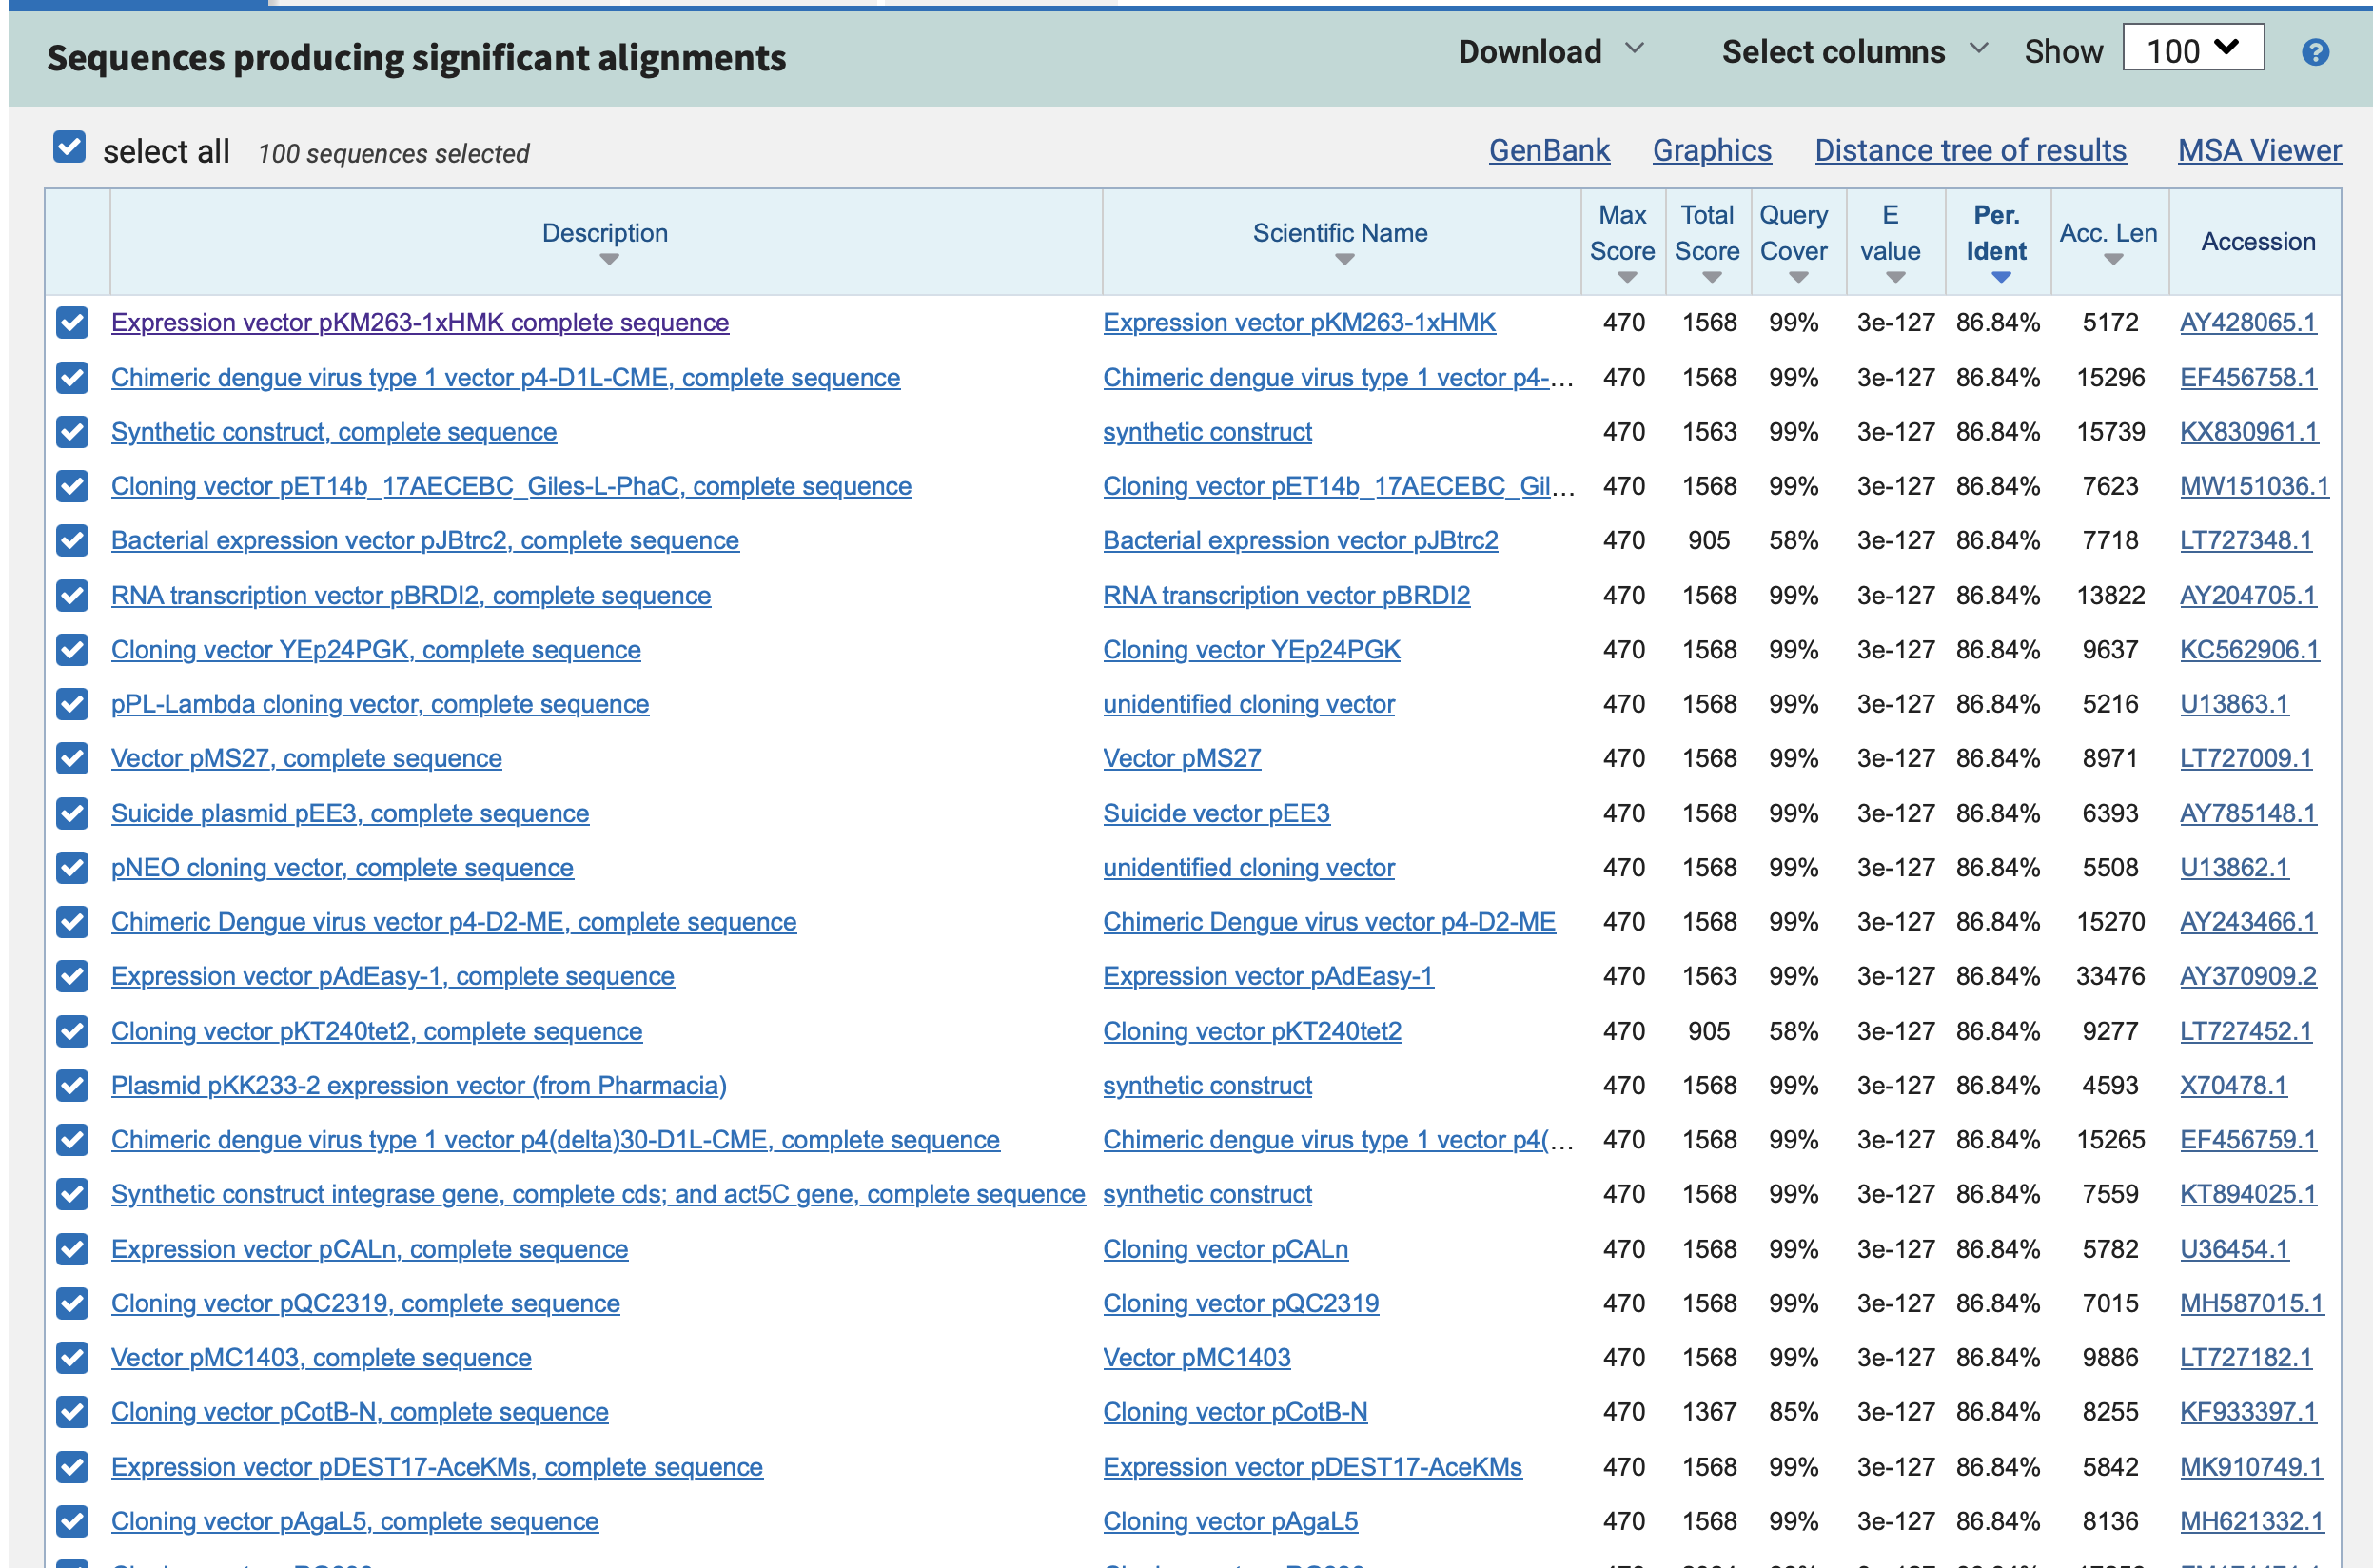
\includegraphics[width=1\textwidth]{q1.png}
\end{figure}


\textbf{There are several matched gene sequence have the same best results. The `Total Score' is 1568; the `Query Cover' is 99\%; The ‘E Value’ is 3e-127; The ‘Per. Ident’ is 86.84\%. After checking the source of these matched gene sequences, we are able to find that most of the results are plasmid sequences. 
It’s likely that this gene has been inserted into plasmid vectors for research purposes, such as cloning, expression, or gene transfer experiments.
}  %加粗字体

\section{Question2}

Mark's published article was brought to Michael Crichton's attention. In his second book, ``The Lost World'', 
Mr. Crichton used Mark as a consultant. 

Here is the sequence Mark gave Michael Crichton for the book ``The Lost World'': 

>LostWorld DinoDNA from the book The Lost World

gaattccgga agcgagcaag agataagtcc tggcatcaga tacagttgga gataaggacg\\
gacgtgtggc agctcccgca gaggattcac tggaagtgca ttacctatcc catgggagcc\\
atggagttcg tggcgctggg ggggccggat gcgggctccc ccactccgtt ccctgatgaa\\
gccggagcct tcctggggct gggggggggc gagaggacgg aggcgggggg gctgctggcc\\
tcctaccccc cctcaggccg cgtgtccctg gtgccgtggg cagacacggg tactttgggg\\
accccccagt gggtgccgcc cgccacccaa atggagcccc cccactacct ggagctgctg\\
caaccccccc ggggcagccc cccccatccc tcctccgggc ccctactgcc actcagcagc\\
gggcccccac cctgcgaggc ccgtgagtgc gtcatggcca ggaagaactg cggagcgacg\\
gcaacgccgc tgtggcgccg ggacggcacc gggcattacc tgtgcaactg ggcctcagcc\\
tgcgggctct accaccgcct caacggccag aaccgcccgc tcatccgccc caaaaagcgc\\
ctgcgggtga gtaagcgcgc aggcacagtg tgcagccacg agcgtgaaaa ctgccagaca\\
tccaccacca ctctgtggcg tcgcagcccc atgggggacc ccgtctgcaa caacattcac\\
gcctgcggcc tctactacaa actgcaccaa gtgaaccgcc ccctcacgat gcgcaaagac\\
ggaatccaaa cccgaaaccg caaagtttcc tccaagggta aaaagcggcg ccccccgggg\\
gggggaaacc cctccgccac cgcgggaggg ggcgctccta tggggggagg gggggacccc\\
tctatgcccc ccccgccgcc ccccccggcc gccgcccccc ctcaaagcga cgctctgtac\\
gctctcggcc ccgtggtcct ttcgggccat tttctgccct ttggaaactc cggagggttt\\
tttggggggg gggcgggggg ttacacggcc cccccggggc tgagcccgca gatttaaata\\
ataactctga cgtgggcaag tgggccttgc tgagaagaca gtgtaacata ataatttgca\\
cctcggcaat tgcagagggt cgatctccac tttggacaca acagggctac tcggtaggac\\
cagataagca ctttgctccc tggactgaaa aagaaaggat ttatctgttt gcttcttgct\\
gacaaatccc tgtgaaaggt aaaagtcgga cacagcaatc gattatttct cgcctgtgtg\\
aaattactgt gaatattgta aatatatata tatatatata tatatctgta tagaacagcc\\
tcggaggcgg catggaccca gcgtagatca tgctggattt gtactgccgg aattc

Select, copy, and paste the ``Lost World'' sequence into NCBI BLAST web portal to run blastx.
Can you find Mark's hidden message? Hine: look at the best pairwise alignment. (3 pts)

\begin{figure}[H] % h:here 就在这个位置插图
    \centering
    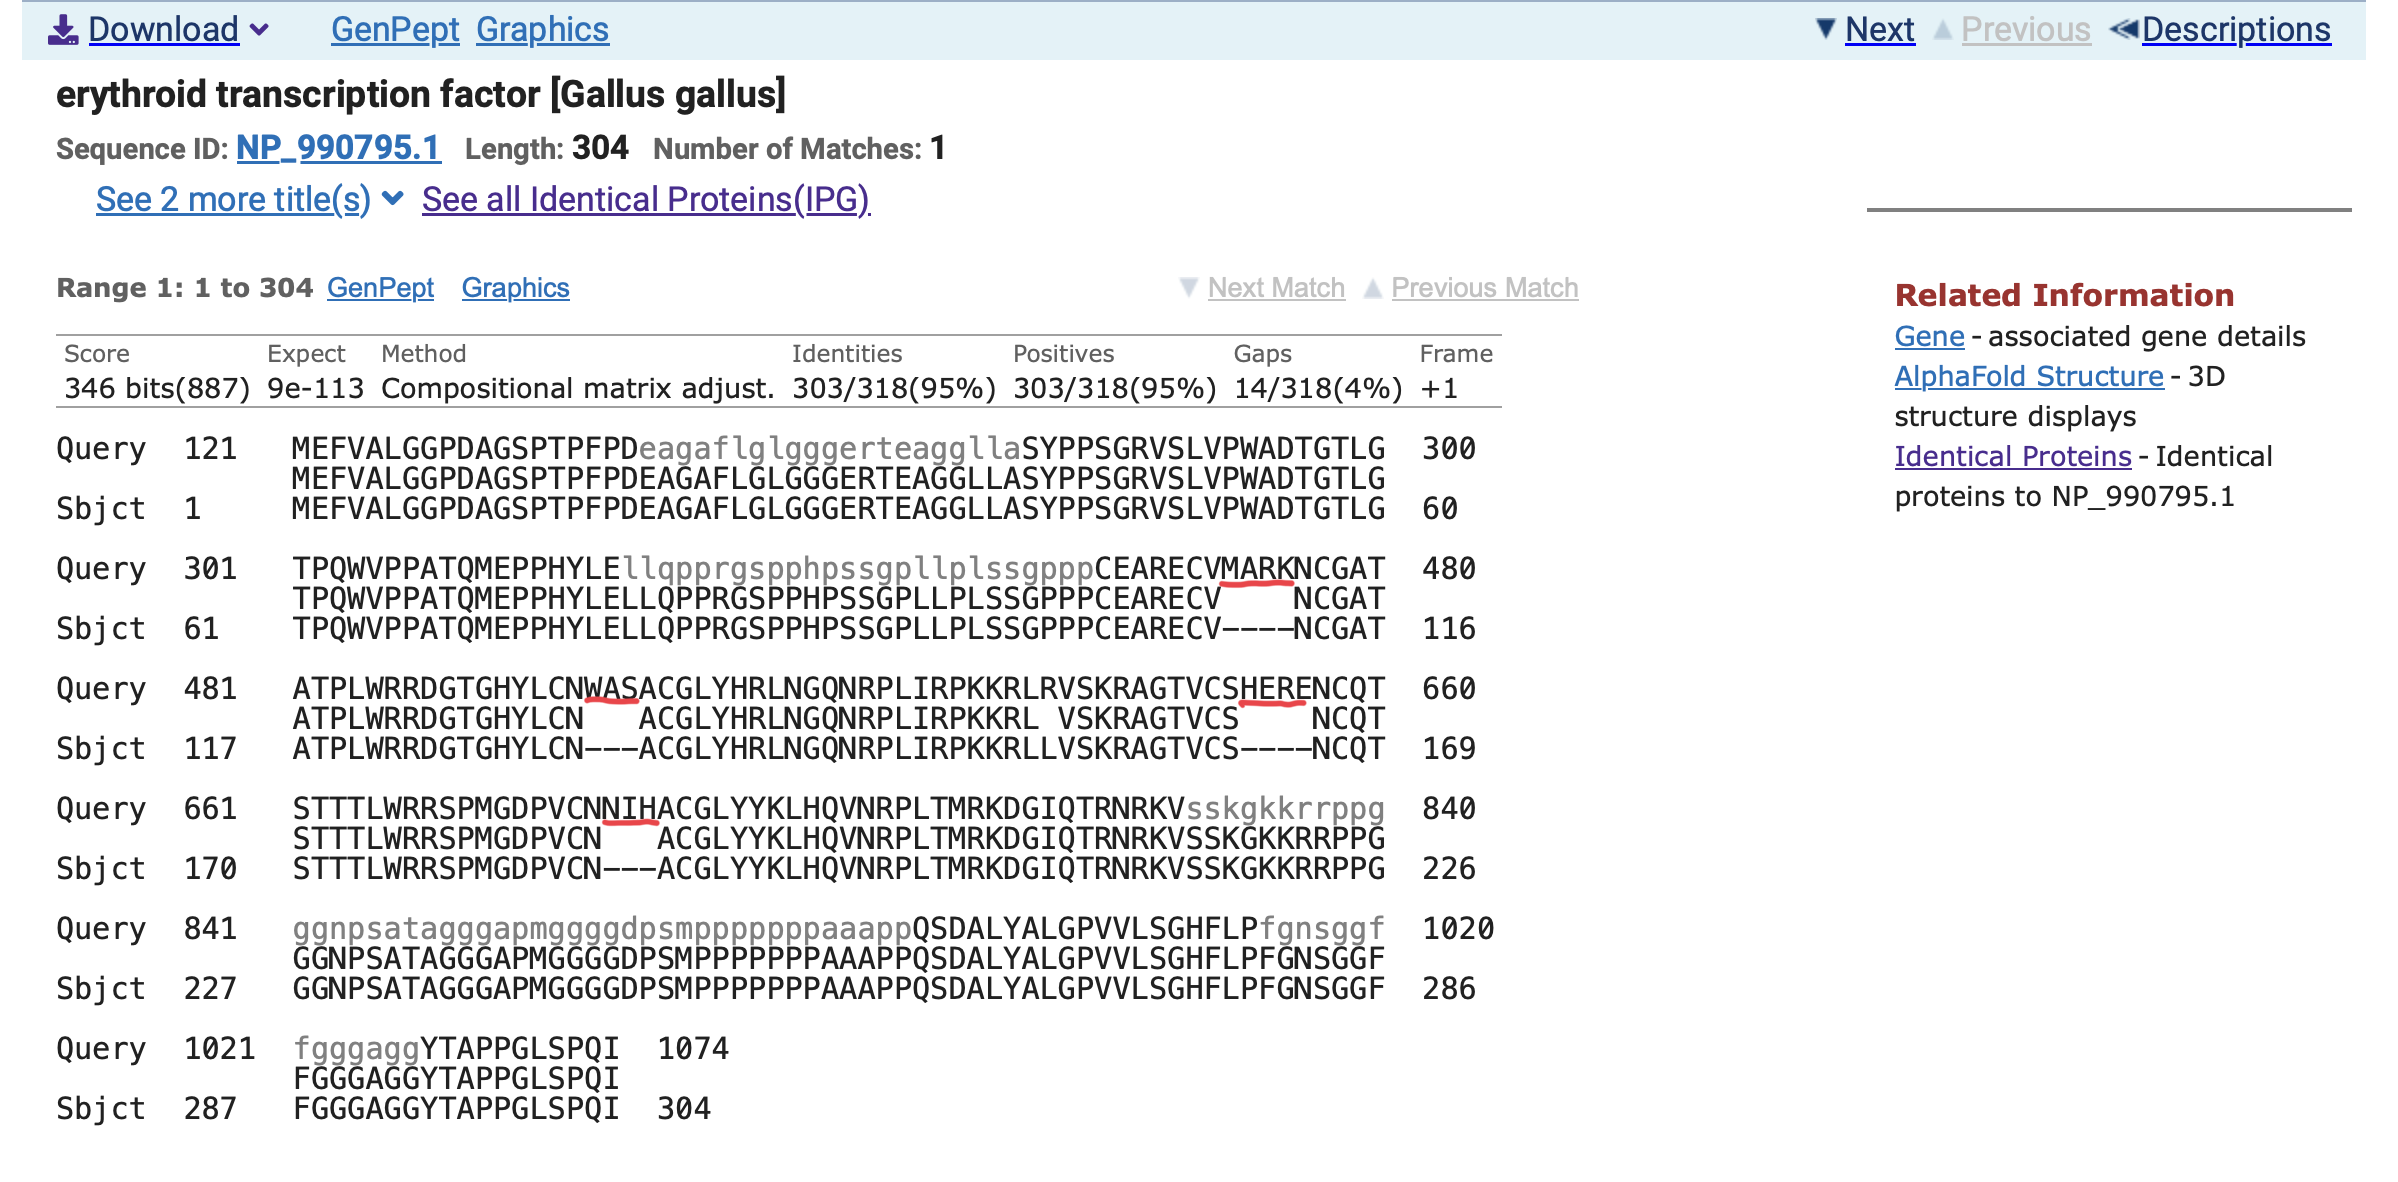
\includegraphics[width=1\textwidth]{q2.png}  % 替换为你的图片文件名

\end{figure}

\textbf{Looking at the best pairwise alignment, we can find that Mark's hidden massage is ``MARK WAS HERE NIH''}

\textbf{Also, the result shows that the best matched sequence refers to a protein called GATA-1(erythroid transcription factor) from Gallup gallus (chicken). GATA-1 is a critical transcription factor involved in the regulation of genes necessary for erythropoiesis (the production of red blood cells).
}

\section{Question3}
Pairwise global alignment. Suppose the alignment scoring function is the following:
Match = 1; mismatch = -3, gap = -4. 

	Suppose the two DNA sequences are 
	
    ATGGTCT
	ACGGTTCT

    \begin{itemize} %无标号列表
        \item Align these two sequences using the Needleman-Wunsch algorithm manually by filling in the table below and show the optimal path. (3pts)
        \item Use Smith-Waterman algorithm to perform a local alignment and show the path. (3 pts)

\end{itemize}

\begin{figure}[H] % h:here 就在这个位置插图
    \centering
    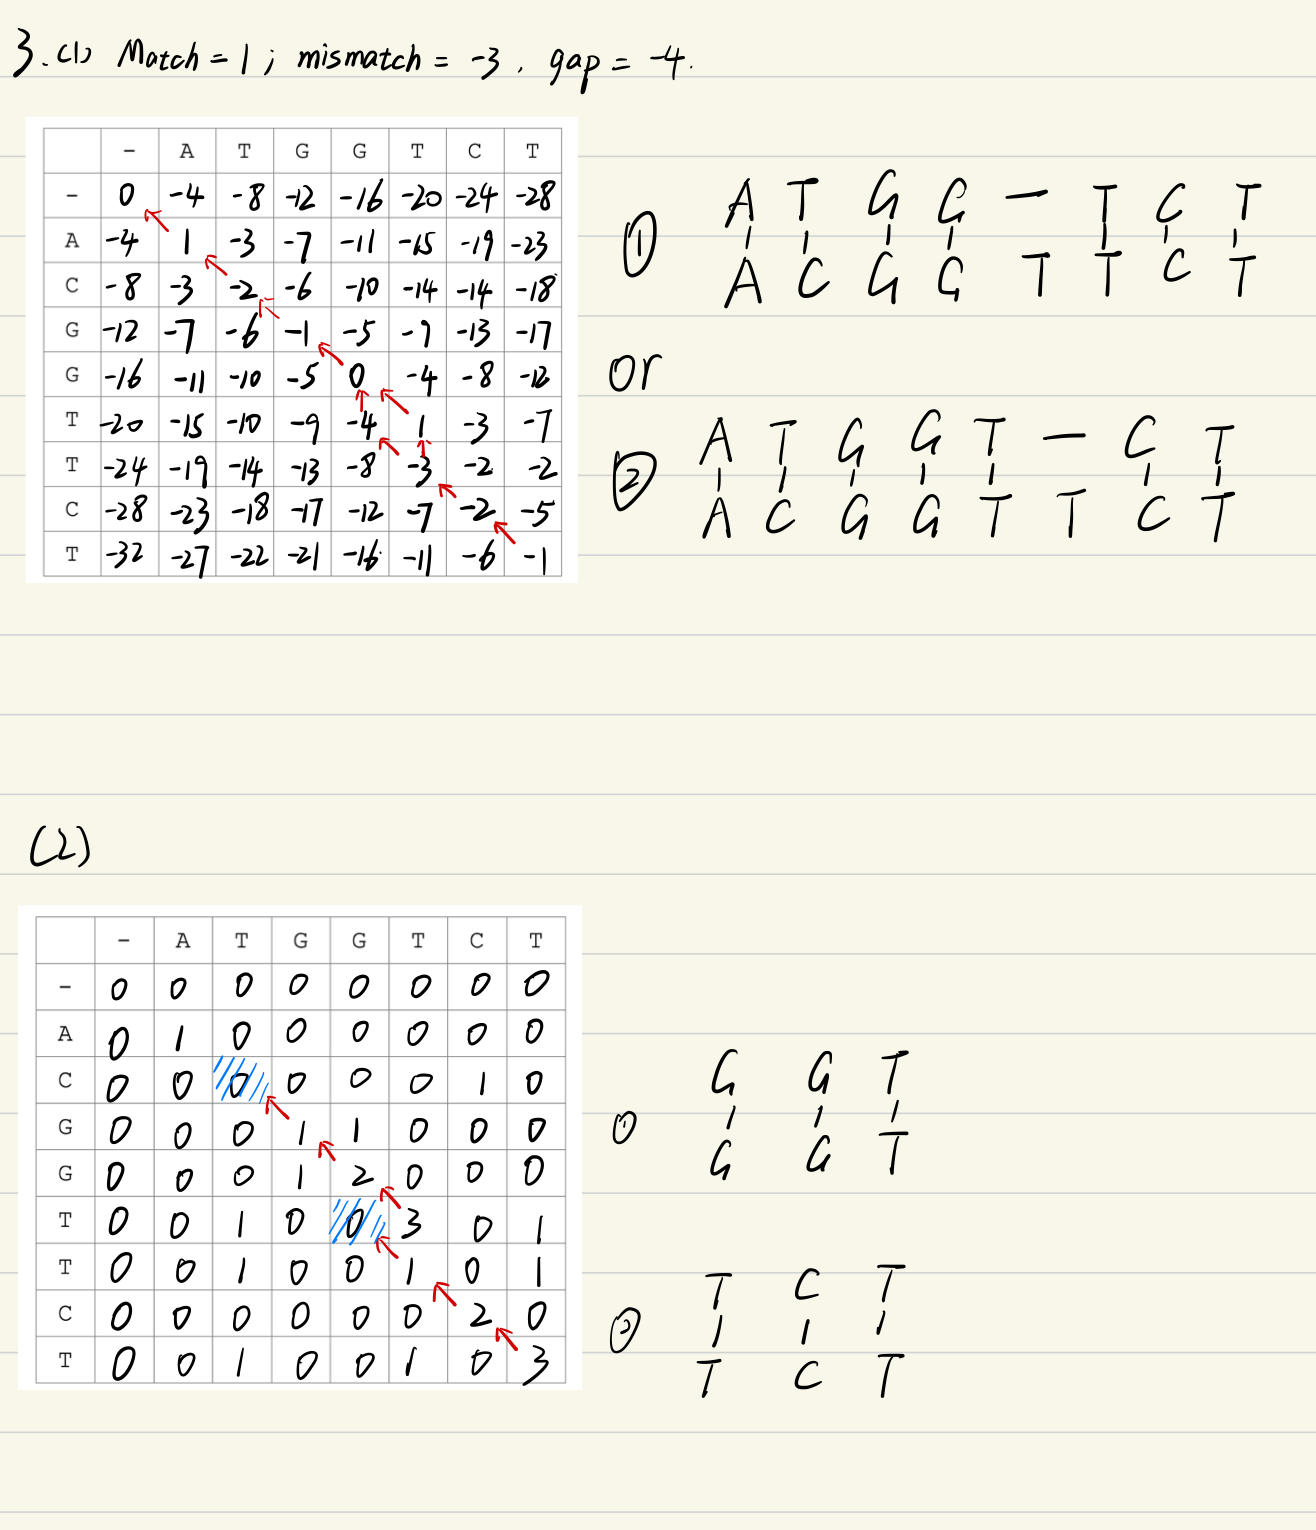
\includegraphics[width=1\textwidth]{q3answer.jpeg}  % 替换为你的图片文件名

\end{figure}


\section{Question4}
Hidden Markov model. Consider a two-state HMM: A (enrichment of A nucleotide) and B (background). 
The emission and transition probabilities are


\centering %后面的输入都会居中
\begin{tabular}{|c|c|}
    \hline
    A\\
    \hline
    A  0.4 \\
    C  0.2  \\
    G  0.2\\
    T  0.2\\
    \hline
\end{tabular}
\begin{tabular}{|c|c|}
    \hline
    B\\
    \hline
    A  0.25 \\
    C  0.25  \\
    G  0.25\\
    T  0.25\\
    \hline
\end{tabular}





\begin{tabular}{|c|c|c|}
    \hline
    &A&B\\
    \hline
    A & 0.5 &0.5\\
    \hline
    b & 0.2&0.8  \\
    \hline
\end{tabular}

\raggedright %靠右开始输出
And the start probabilities for both states are 0.5.

Please infer the hidden states of sequence “GAATACGA” using the Viterbi algorithm. 
Please show your steps. (3 pts)
% 定义代码背景颜色



\begin{figure}[H]
    \centering
    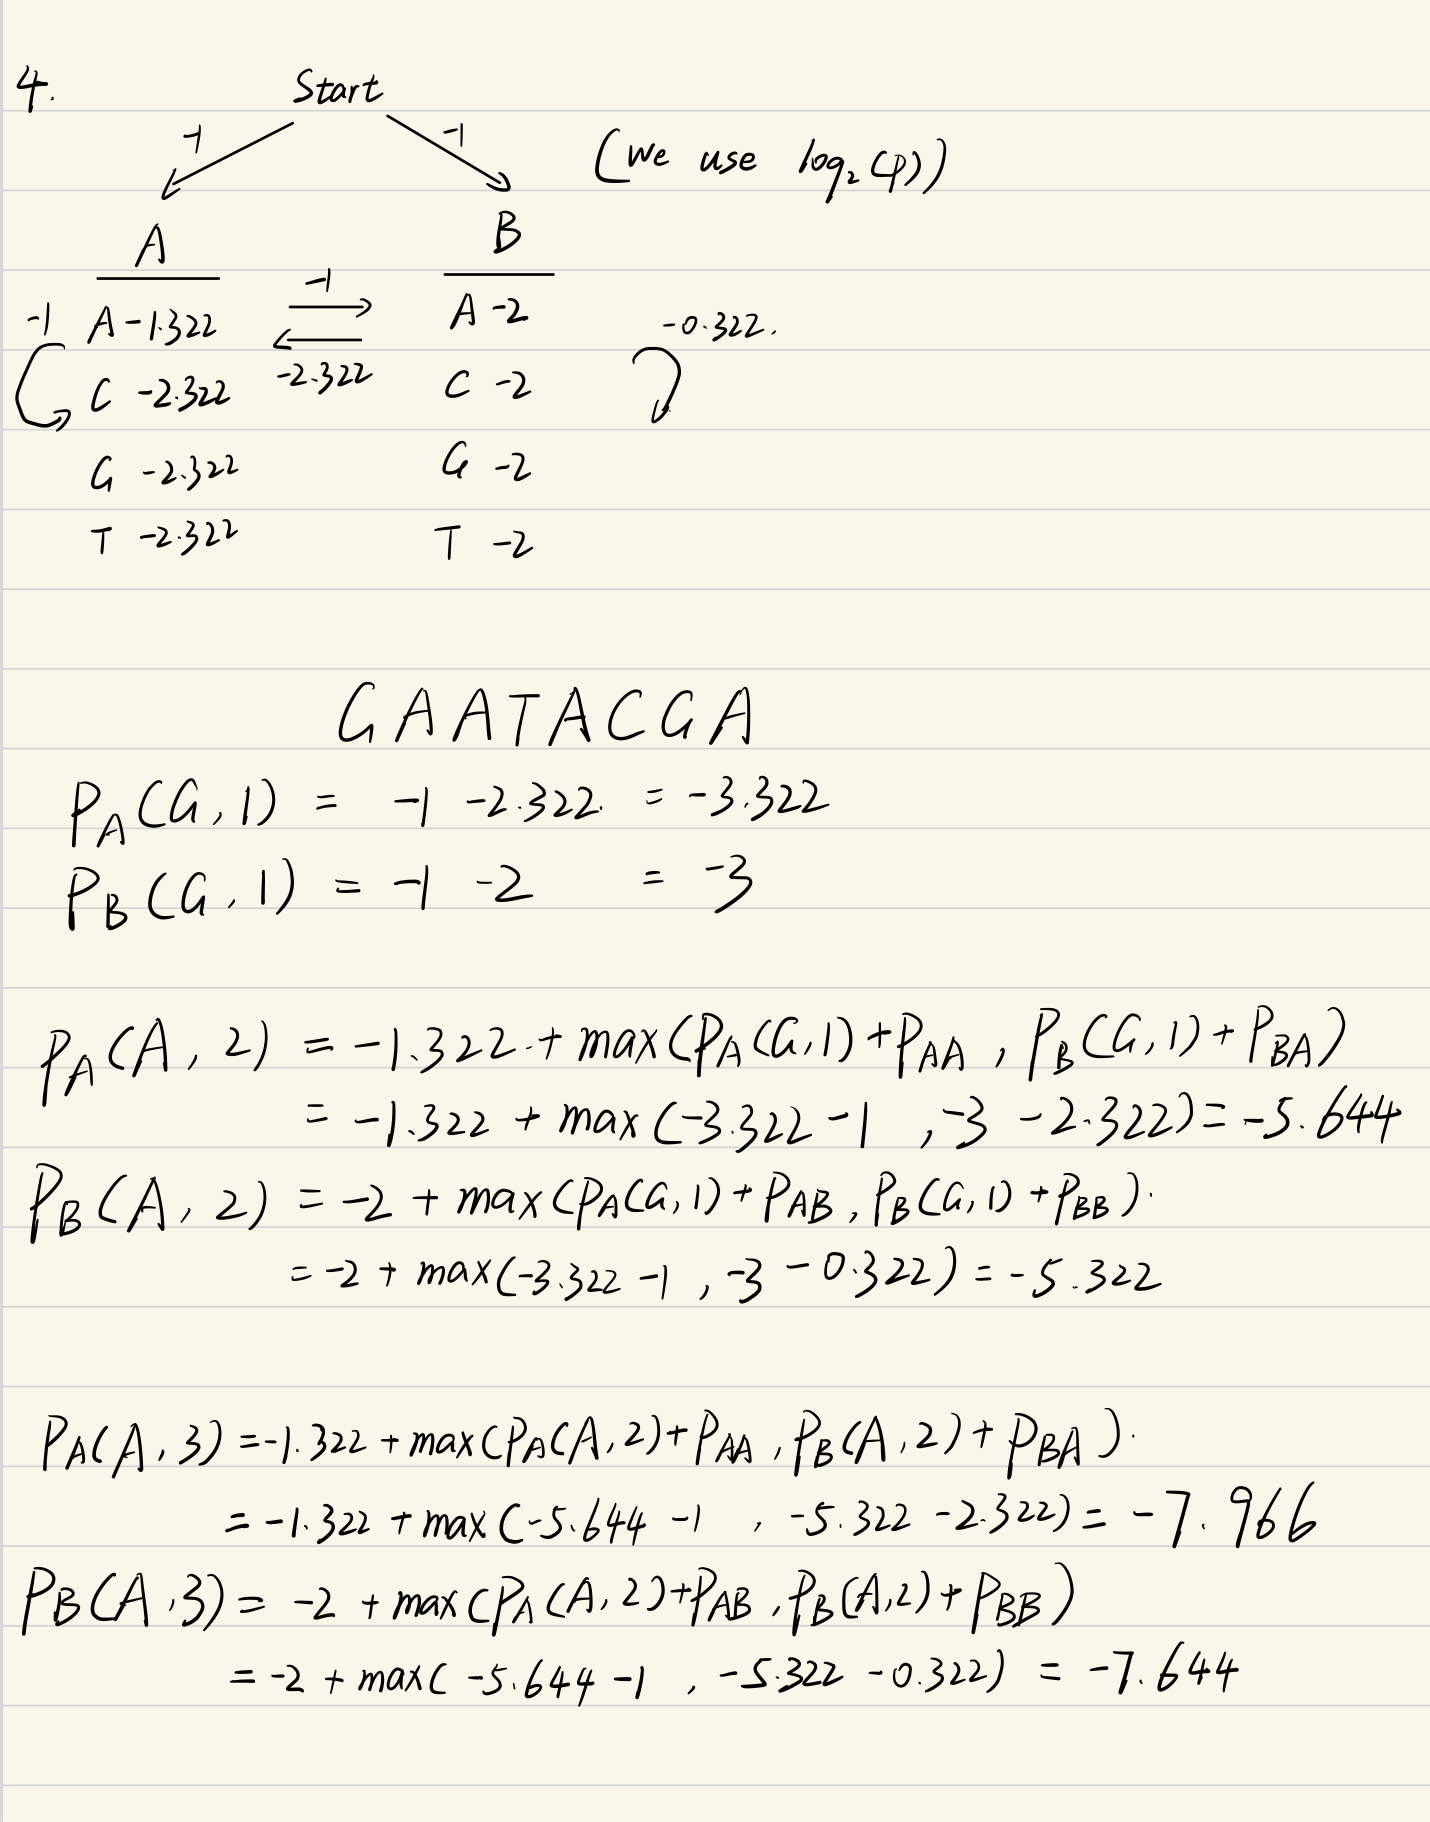
\includegraphics[width=0.9\textwidth]{q4answer.jpeg}  % 替换为你的图片文件名

\end{figure}

\textbf{Sometimes the sequence is long. Calculating by hand is inconvenient. We can use python to solve this.
Here is the code:
}




\begin{center}
    %加代码格
    \begin{lstlisting} 
import numpy as np

def viterbi(obs, states, start_p, trans_p, emit_p):
    # obs: observation sequence
    # states: hidden states
    # start_p: initial probabilities
    # trans_p: state transition probabilities
    # emit_p: emission probabilities   
    # Initialize variables
    V = [{}]  # Viterbi table, V[t][s] represents the maximum probability of being in state s at time t
    path = {}  # To save the optimal path
    
    # Initialize the Viterbi table for t=0
    for s in states:
        V[0][s] = start_p[s] * emit_p[s][obs[0]]
        path[s] = [s]
    
    # Update the Viterbi table for each time step t
    for t in range(1, len(obs)):
        V.append({})
        new_path = {}

        for s in states:
            # Select the optimal previous state, meaning which previous state is most likely to result in the current observation and state
            (prob, state) = max((V[t-1][prev_state] * trans_p[prev_state][s] * emit_p[s][obs[t]], prev_state) for prev_state in states)
            V[t][s] = prob
            new_path[s] = path[state] + [s]
        
        path = new_path

    # Termination: Select the optimal path for the last time step
    (prob, state) = max((V[len(obs) - 1][s], s) for s in states)
    return prob, path[state], V

# Example data
states = ('A', 'B')
observations = ('G', 'A', 'A', 'T', 'A', 'C', 'G', 'A')
start_probability = {'A': 0.5, 'B': 0.5}
transition_probability = {
   'A': {'A': 0.5, 'B': 0.5},
   'B': {'A': 0.2, 'B': 0.8},
}
emission_probability = {
   'A': {'A': 0.4, 'C': 0.2, 'G': 0.2, 'T': 0.2},
   'B': {'A': 0.25, 'C': 0.25, 'G': 0.25, 'T': 0.25},
}

# Run the Viterbi algorithm
prob, optimal_path, V = viterbi(observations, states, start_probability, transition_probability, emission_probability)
print(f"Optimal path: {optimal_path}")
print(f"Maximum probability: {prob}")
print(V)
\end{lstlisting}
\end{center}
\textbf{We get:}



\begin{figure}[H]
    \centering
    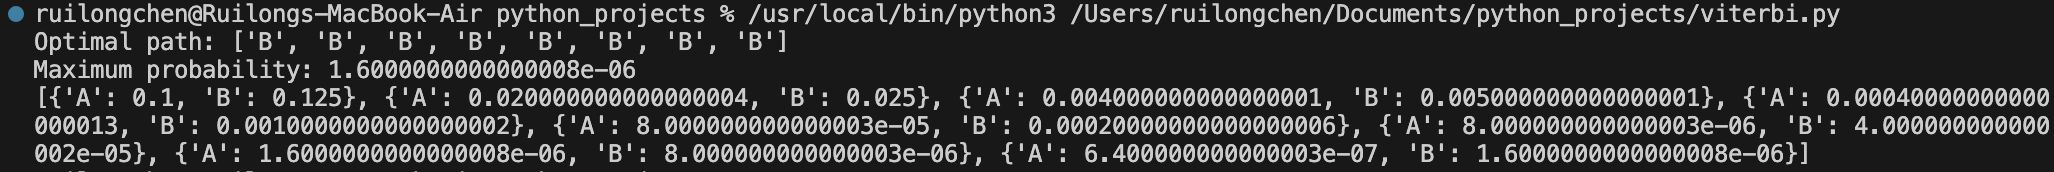
\includegraphics[width=1\textwidth]{coderesult.jpg}  % 替换为你的图片文件名
\end{figure}

\begin{tabular}{|c|c|c|c|c|c|c|c|c|}
    \hline
    &G&A&A&T&A&C&G&A\\
    \hline
    A & 0.1 &0.02 &0.004& 0.0004&$8 \times 10^{-5} $& $8 \times 10^{-6}$& $1.6 \times 10^{-6}$& $6.4 \times 10^{-7}$\\
    \hline
    B& 0.125 &0.025 &0.005& 0.001&0.0002 & $4 \times 10^{-5}$& $8 \times 10^{-6}$& $1.6 \times 10^{-6}$\\
    \hline
\end{tabular}


\textbf{The most probable path is: BBBBBBBB. The probability is: $1.6 \times 10^{-6}$.
}

\section{Question5}

CTCF (CCCTC-binding factor) is a zinc-finger protein that functions as a transcription factor. It also has insulator activity and is important for the 3D structure of chromatin, through formation of chromatin loops. Using the frequency matrix found at JASPAR using ID MA0139.1
\begin{itemize}
    \item Represent the CTCF motif using IUPAC code (assume a nucleotide is absent from a position if its proportion is less than 10\%. (1 pt)

\end{itemize}

Read Stormo and Hartzell PNAS 1989 paper (can be found in the references folder under Files of the course Canvas website. Generate Fig 1 B, C and D using the CTCF frequency matrix from the above.

\begin{itemize}
    \item Fig 1B. Derive the position-specific weight matrix (PSWM). (2 pts) 
    \item Fig 1C. Derive the specific matrix. Note that the number “23” used in the calculation 0.5/23 when fb = 0 need to be modified for CTCF. You need to figure out what number should be used. Also use pb = 0.25 for all b. (2 pts)
    \item Fig 1D. Draw Iseq for CTCF (hand draw is fine). (2 pts)
    \item Fig 1D. What is the sum of all positions for CTCF (in bits)? (1 pt)
\end{itemize}


%插入链接
Simulate 10 CTCF motifs using the PSWM, i.e., generate 10 CTCF motif sequences. Put them in FASTA format, use weblogo web server \href{http://weblogo.threeplusone.com/}{http://weblogo.threeplusone.com/} to generate a logo plot. (1 pt)


\textbf{We can find the frequency matrix at JASPAR:}

\begin{figure}[h]
    \centering
    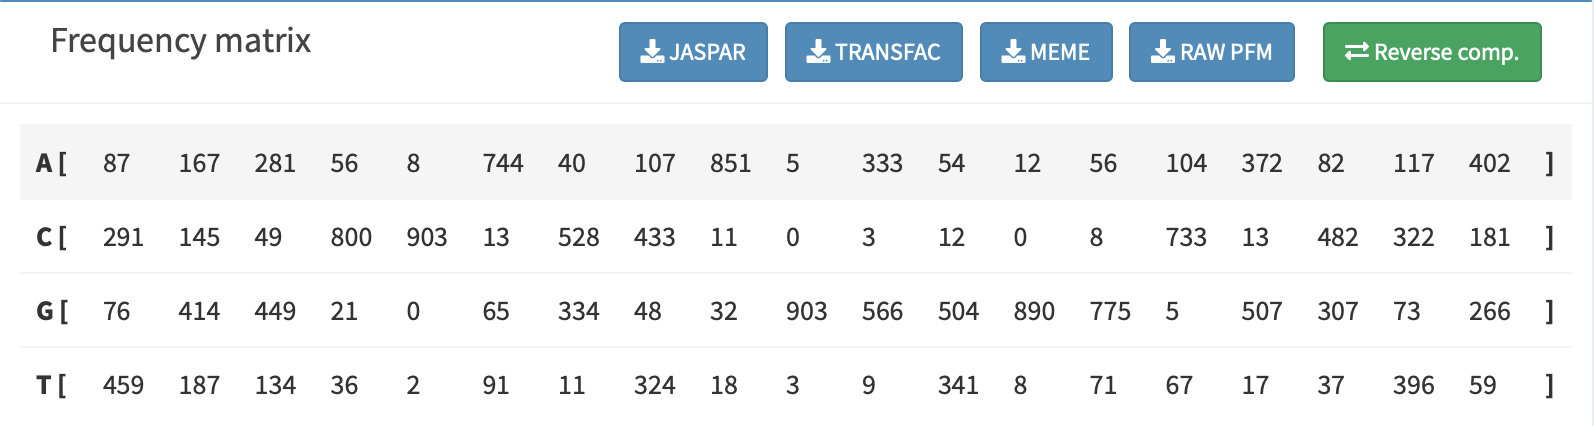
\includegraphics[width=1\textwidth]{jasparfreqmatrix.png}  % 替换为你的图片文件名
\end{figure}

\textbf{Then we can calculate the proportion, and assume a nucleotide is absent if its 
proportion is less than 10\%}

\begin{figure}[H]
    \centering
    
    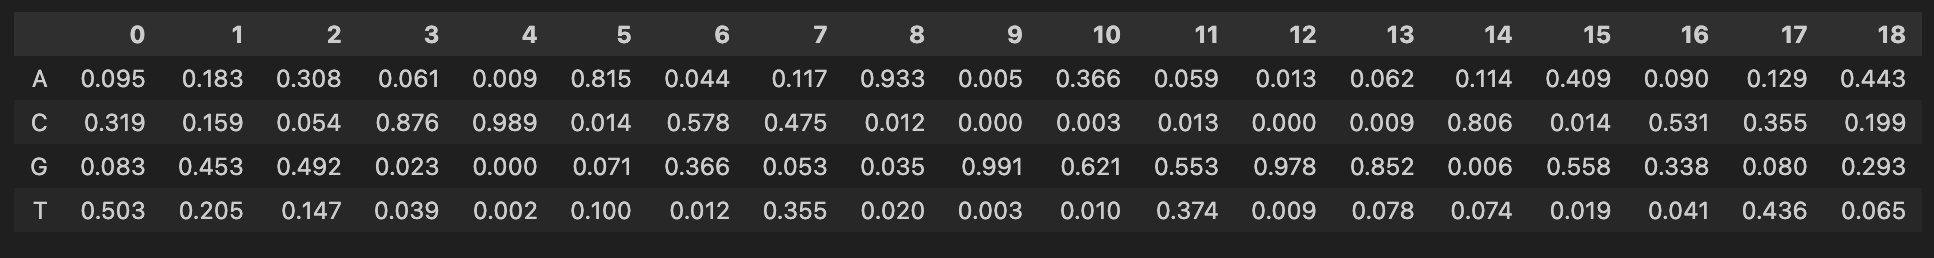
\includegraphics[width=1\textwidth]{pythonfreq1.png}  % 替换为你的图片文件名
    \caption{PSWM}
\end{figure}

\begin{figure}[H]
    \centering
    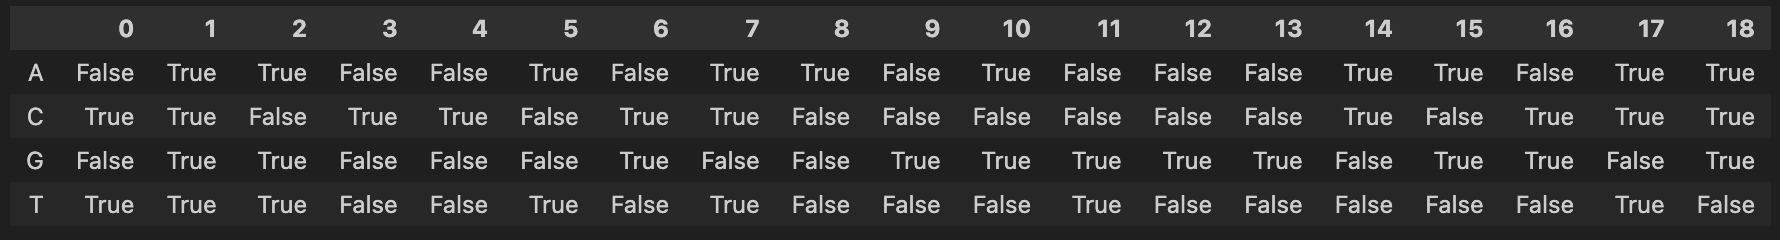
\includegraphics[width=1\textwidth]{pythonfreq2.png}  % 替换为你的图片文件名
\end{figure}

\textbf{Finally, we can use IUPAC code to represent the motif: 
}

\textbf{YNDCCWSHAGRKGGMRSHV
}

\textbf{We have gained the PSWM, we can then calculate the specific matrix. At positions
for which $ f_b = 0 $, we use 0.5/20 to estimate the frequency. The specific matrix is 
calculated as $log_2(f_b / p_b)$. We can get:}


\begin{figure}[H]
    \centering
    
    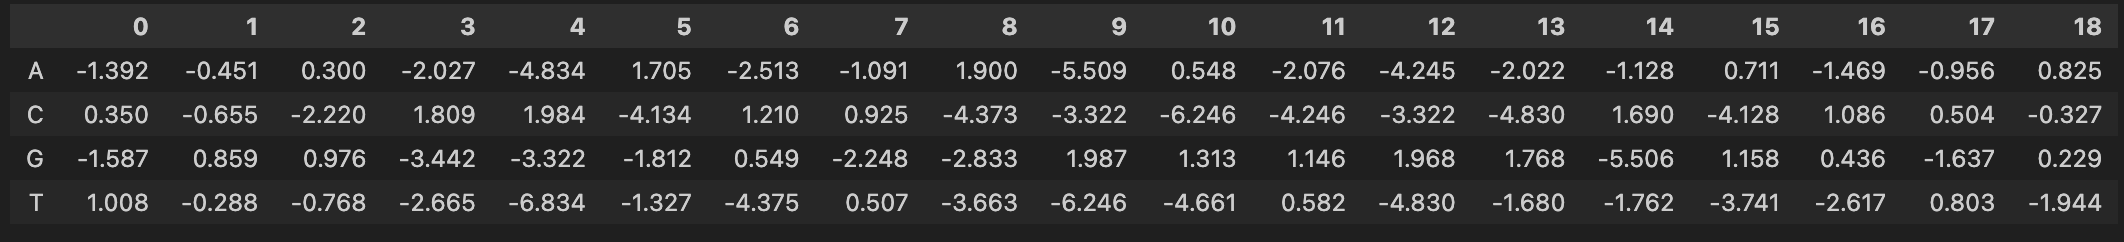
\includegraphics[width=1\textwidth]{specificmatrix.png}  % 替换为你的图片文件名
    \caption{specific matrix}
\end{figure}

\textbf{Then, use $I_{seq} =  \sum_{b=A}^T f_b log_2 (\frac{f_b}{p_b})$ to calculate the $I_{seq}$ and draw it:
}

\begin{figure}[H]
    \centering
    % 左边图片
    \begin{minipage}{0.15\textwidth}
        \centering
        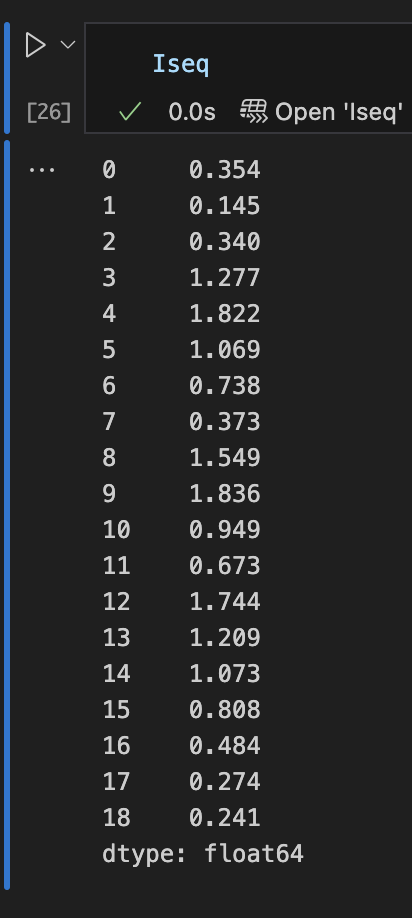
\includegraphics[width=\textwidth]{Iseq.png}

    \end{minipage}
    \hfill  % 增加水平间隔
    % 右边图片
    \begin{minipage}{0.8\textwidth}
        \centering
        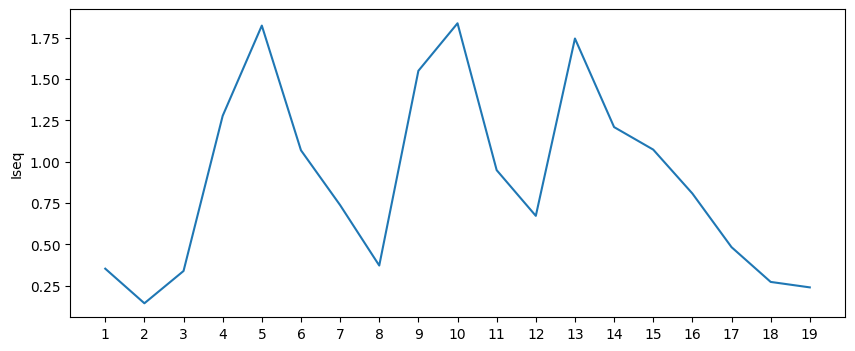
\includegraphics[width=1\textwidth]{Iseqplot.png}

    \end{minipage}
    \caption{Iseq}
\end{figure}

\textbf{So, the sum of all positions is 16.96 bits.}

\textbf{We use python to do the simulation:}
\begin{center}
    \begin{lstlisting}
import pandas as pd
import numpy as np
A = [87,167,281,56,8,744,40,107,851,5,333,54,12,56,104,372,82,117,402]
C = [291, 145, 49, 800, 903, 13, 528, 433, 11, 0 , 3, 12, 0 ,8, 733, 13, 482, 322,181]
G = [76, 414, 449 , 21, 0 ,65, 334, 48, 32, 903, 566, 504, 890, 775, 5, 507, 307, 73, 266]
T = [459, 187, 134, 36 , 2, 91,11,324,18,3,9,341,8,71,67,17,37,396,59]

df=pd.DataFrame({'A':A, 'C':C,'G':G,'T':T})
ctcf_pswm=df.divide(df.sum(axis=1),axis=0)

# Define the nucleotides and create a function to generate a sequence based on the PSWM
nucleotides = ['A', 'C', 'G', 'T']

def generate_sequence(pswm, length):
    sequence = []
    for i in range(length):
        # Choose a nucleotide based on the PSWM probabilities for the current position
        nucleotide = np.random.choice(nucleotides, p=pswm.iloc[i])
        sequence.append(nucleotide)
    return ''.join(sequence)

# Simulate 10 motifs
motifs = [generate_sequence(ctcf_pswm, ctcf_pswm.shape[0]) for _ in range(10)]

# Write motifs to FASTA format
with open('ctcf_motifs.fasta', 'w') as fasta_file:
    for i, motif in enumerate(motifs):
        fasta_file.write(f">motif_{i+1}\n{motif}\n")
    \end{lstlisting}
\end{center}

\textbf{Put file into the website, we get:}


\begin{figure}[H]
    \centering
    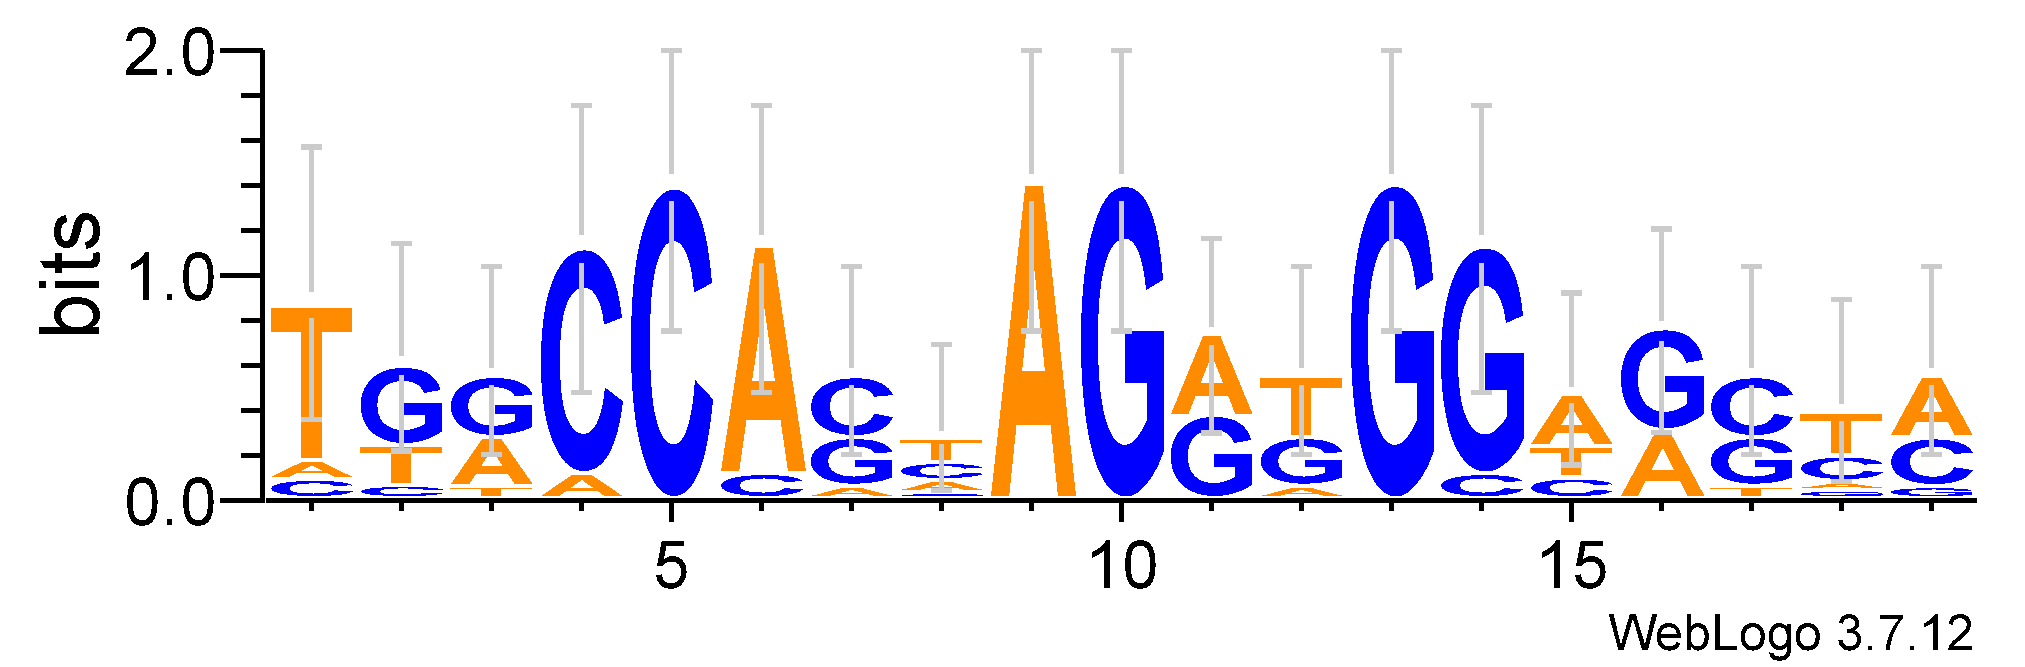
\includegraphics[width=1\textwidth]{logo.png}
\end{figure}

\section{Question6}
Locate the FOXA2 motif using JASPAR ID MA0047.4. Using the motif’s PSWM to can the motif against the following sequence:

ACGTGCTAAG

Write down the matching probability for all possible motif start positions. Show your work. (3 pts).


\begin{figure}[H]
    \centering
    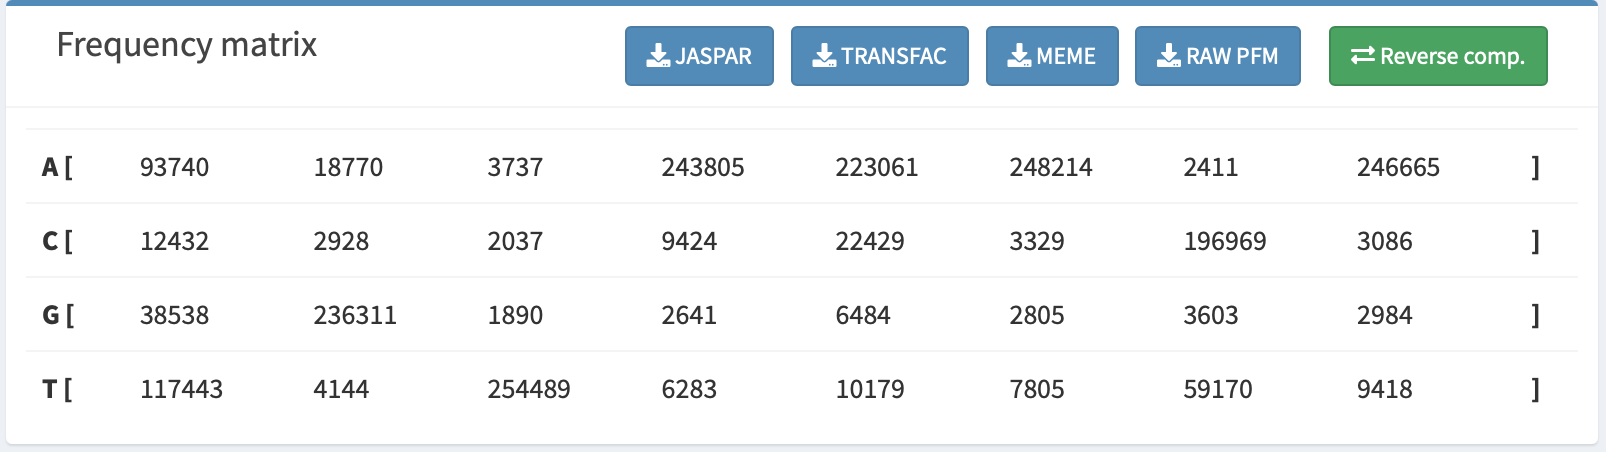
\includegraphics[width=1\textwidth]{q6.png}

\end{figure}

\begin{figure}[H]
    \centering
    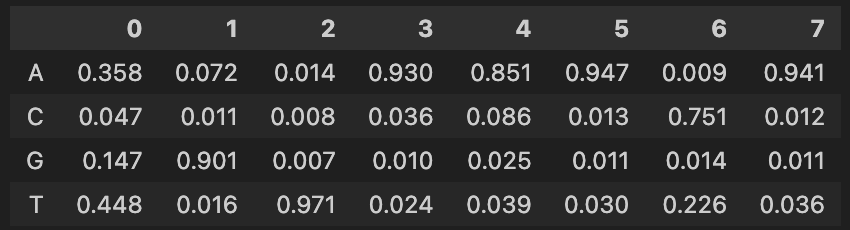
\includegraphics[width=1\textwidth]{q6freq.png}

\end{figure}

\textbf{
There are 3 start positions, denote as $ S_1$,$S_2$,$S_3$.}

$P(S_1) = 0.358 *  0.011 *  0.007 * 0.024 *0.025 * 0.013 *0.226 * 0.941 \approx 4.57 * 10^{-11}$ 

$P(S_2) = 0.047 *  0.901 *  0.971 * 0.01 *0.086 * 0.030 *0.009 * 0.941 \approx 8.98 * 10^{-9}$ 

$P(S_3) = 0.147 *  0.016 *  0.007 * 0.036 *0.039 * 0.947 *0.009 * 0.011 \approx 2.17* 10^{-12} $ 

\section{Quesion7}

Given the snapshot of called peaks from a TF ChIP-seq experiment in a part of the genome below. Suppose a colored triangle indicates a motif site. Please indicate which motif (color) is likely to be the binding site of the TF and explain why? (3 pts)


\begin{figure}[H]
    \centering
    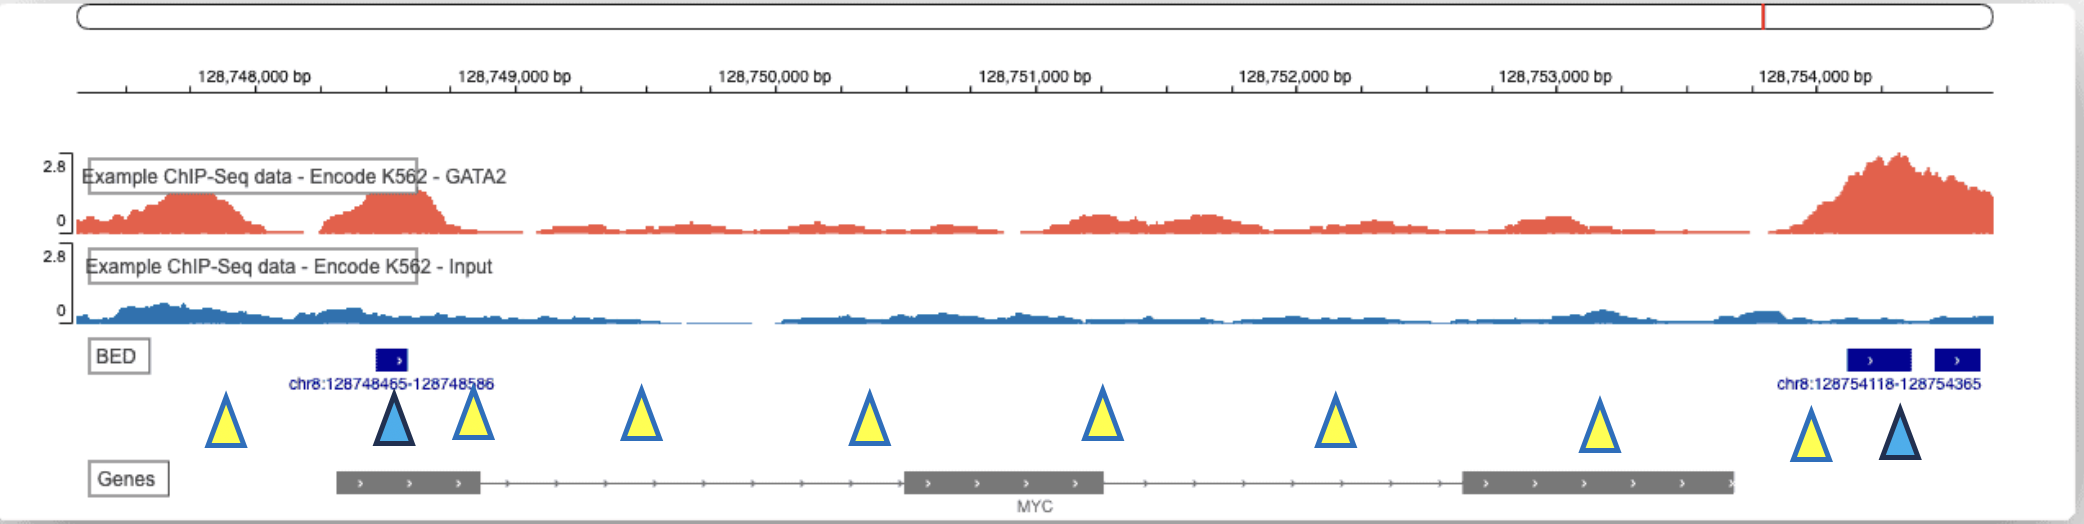
\includegraphics[width=1\textwidth]{q7.png}
\end{figure}


\textbf{The blue triangle likely represents the binding site of the transcription factor because it is positioned directly under the highest ChIP-seq peak, which is indicative of strong TF-DNA binding activity. }

\end{document}